\documentclass{article}[18pt]
\usepackage[utf8]{inputenc}
\usepackage[margin=0.7in]{geometry}
\usepackage{parselines} 
\usepackage{amsmath}
\usepackage{titlesec}
\usepackage{pgfplots}
\usepackage{graphicx}
\usepackage[english]{babel}
\usepackage{fancyhdr}
\usepackage{amssymb}
\pgfplotsset{width=10cm,compat=1.9}
\usepackage{mwe}
\usepackage{float}
\usepackage{tabularx}
\usepackage{tikz}
\usetikzlibrary{calc,trees,positioning,arrows,fit,shapes,calc,decorations.markings}
\tikzset{->-/.style={decoration={
  markings,
  mark=at position .5 with {\arrow{>}}},postaction={decorate}}}
\titlespacing\section{0pt}{14pt plus 4pt minus 2pt}{0pt plus 2pt minus 2pt}
\newlength\tindent
\setlength{\tindent}{\parindent}
\setlength{\parindent}{0pt}
\renewcommand{\indent}{\hspace*{\tindent}}

\pagestyle{fancy}
\fancyhf{}
\rhead{Sam Robbins 13SE}
\lhead{A Level Maths - C3}
\rfoot{Page \thepage}

\newcommand{\R}{\mathbb{R}}
\pgfplotsset{ytick style={draw=none}}
\pgfplotsset{xtick style={draw=none}}


\begin{document}
\begin{center}
\underline{\huge C3}
\end{center}
\section{Algebraic fractions}
Algebraic fractions can be simplified by equating the fraction to an equation made of constants
\subsection{Example}
$\dfrac{x^3+2x^2-6x+1}{x-1}\equiv Ax^2+Bx+C+\dfrac{D}{x-1}$\\
\\
\\
$x^3+2x^2-6x+1\equiv(x-1)(Ax^2+Bx+C)+D$\\
\\
$x^3+2x^2-6x+1\equiv Ax^3+(B-A)x^2+(C-B)x+(D-C)1$\\
\\
\begin{tabularx}{\textwidth}{|X|X|X|}
\hline
Term&Calculation&Final Value\\
\hline
$x^3$ coefficient&$1=A$&$\mathbf{A=1}$\\
\hline
$x^2$ coefficient&$2=B-A$&$\mathbf{B=3}$\\
\hline
$x$ coefficient&$-6=C-B$&$\mathbf{C=-3}$\\
\hline
Constant term&$1=D-C$&$\mathbf{D=-2}$\\
\hline
\end{tabularx}
\\
\\
\\
$x^2+3x-3+\dfrac{-2}{x-2}$
\section{Functions}
\subsection{Definitions}
\textbf{Domain} - The input to a function\\
\textbf{Range} - The output from a function
\subsection{Function mapping}


\begin{figure}[h]
    \centering
    \begin{minipage}{0.28\textwidth}
        \centering
         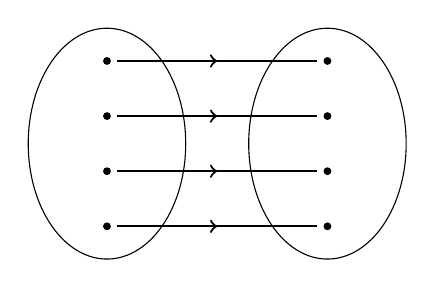
\begin{tikzpicture}[ele/.style={fill=black,circle,minimum width=.8pt,inner sep=1pt},every fit/.style={ellipse,draw,inner sep=-2pt},scale=0.7]
  \node[ele,] (a1) at (0,4) {};    
  \node[ele,] (a2) at (0,3) {};    
  \node[ele,] (a3) at (0,2) {};
  \node[ele,] (a4) at (0,1) {};

  \node[ele,,] (b1) at (4,4) {};
  \node[ele,,] (b2) at (4,3) {};
  \node[ele,,] (b3) at (4,2) {};
  \node[ele,,] (b4) at (4,1) {};

  \node[draw,fit= (a1) (a2) (a3) (a4),minimum width=2cm] {} ;
  \node[draw,fit= (b1) (b2) (b3) (b4),minimum width=2cm] {} ;  
  \draw[->-,thick,shorten <=2pt,shorten >=2pt] (a1) -- (b1);
  \draw[->-,thick,shorten <=2pt,shorten >=2] (a2) -- (b2);
  \draw[->-,thick,shorten <=2pt,shorten >=2] (a3) -- (b3);
  \draw[->-,thick,shorten <=2pt,shorten >=2] (a4) -- (b4);
 \end{tikzpicture}
        \caption{One-to-one function}
    \end{minipage}\hfill
    \begin{minipage}{0.28\textwidth}
        \centering
                          \begin{tikzpicture}[ele/.style={fill=black,circle,minimum width=.8pt,inner sep=1pt},every fit/.style={ellipse,draw,inner sep=-2pt},scale=0.7]
  \node[ele,] (a1) at (0,4) {};    
  \node[ele,] (a2) at (0,3) {};    
  \node[ele,] (a3) at (0,2) {};
  \node[ele,] (a4) at (0,1) {};

  \node[ele,,] (b1) at (4,4) {};
  \node[ele,,] (b4) at (4,1) {};

  \node[draw,fit= (a1) (a2) (a3) (a4),minimum width=2cm] {} ;
  \node[draw,fit= (b1) (b2) (b3) (b4),minimum width=2cm] {} ;  
  \draw[->-,thick,shorten <=2pt,shorten >=2pt] (a1) -- (b1);
  \draw[->-,thick,shorten <=2pt,shorten >=2] (a2) -- (b1);
  \draw[->-,thick,shorten <=2pt,shorten >=2] (a3) -- (b4);
  \draw[->-,thick,shorten <=2pt,shorten >=2] (a4) -- (b4);
 \end{tikzpicture}
        \caption{Many-to-one function}
    \end{minipage}\hfill
    \begin{minipage}{0.28\textwidth}
        \centering
                          \begin{tikzpicture}[ele/.style={fill=black,circle,minimum width=.8pt,inner sep=1pt},every fit/.style={ellipse,draw,inner sep=-2pt},scale=0.7]
  \node[ele,] (a1) at (0,4) {};    
  \node[ele,] (a4) at (0,1) {};

  \node[ele,,] (b1) at (4,4) {};
  \node[ele,,] (b2) at (4,3) {};
  \node[ele,,] (b3) at (4,2) {};
  \node[ele,,] (b4) at (4,1) {};

  \node[draw,fit= (a1) (a2) (a3) (a4),minimum width=2cm] {} ;
  \node[draw,fit= (b1) (b2) (b3) (b4),minimum width=2cm] {} ;  
  \draw[->-,thick,shorten <=2pt,shorten >=2pt] (a1) -- (b1);
  \draw[->-,thick,shorten <=2pt,shorten >=2] (a1) -- (b2);
  \draw[->-,thick,shorten <=2pt,shorten >=2] (a4) -- (b3);
  \draw[->-,thick,shorten <=2pt,shorten >=2] (a4) -- (b4);
 \end{tikzpicture}
        \caption{Not a function}
    \end{minipage}
\end{figure}
A function is a mapping so that every element of the domain maps to exactly one element of the range
\subsubsection{Changing non functions to functions}
Some non functions can be changed to functions by restricting the domain\\
For example for $f(x)=\sqrt x$ where $x\in\mathbb{R}$ all positive values get mapped, however negative numbers don't, see below:
\begin{figure}[h]
 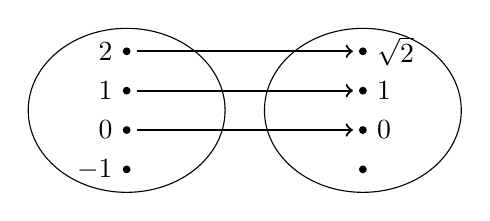
\begin{tikzpicture}[ele/.style={fill=black,circle,minimum width=.8pt,inner sep=1pt},every fit/.style={ellipse,draw,inner sep=-2pt},scale=0.5]
  \node[ele,label=left:$2$] (a1) at (0,4) {};    
  \node[ele,label=left:$1$] (a2) at (0,3) {};    
  \node[ele,label=left:$0$] (a3) at (0,2) {};
  \node[ele,label=left:$-1$] (a4) at (0,1) {};

  \node[ele,,label=right:$\sqrt{2}$] (b1) at (6,4) {};
  \node[ele,,label=right:$1$] (b2) at (6,3) {};
  \node[ele,,label=right:$0$] (b3) at (6,2) {};
  \node[ele,,] (b4) at (6,1) {};

  \node[draw,fit= (a1) (a2) (a3) (a4),minimum width=2.5cm] {} ;
  \node[draw,fit= (b1) (b2) (b3) (b4),minimum width=2.5cm] {} ;  
  \draw[->,thick,shorten <=2pt,shorten >=2pt] (a1) -- (b1);
  \draw[->,thick,shorten <=2pt,shorten >=2] (a2) -- (b2);
  \draw[->,thick,shorten <=2pt,shorten >=2] (a3) -- (b3);
 \end{tikzpicture}
 \end{figure}\\
This means that the domain must be restricted to $x\geqslant0$
\subsection{Inverse functions}
The inverse of $f(x)$ is written as $f^{-1}(x)$\\
The domain and range of inverse function are the opposite of the normal function.
\subsubsection{Finding the inverse function}
To find the inverse function isolate $x$ then replace $x$ with $f^{-1}(x)$ and $y$ with $x$\\
\\
$y=2x^2-7$\\
\\
$y+7=2x^2$\\
\\
$\dfrac{y+7}{2}=x^2$\\
\\
$x=\sqrt{\dfrac{y+7}{2}}$\\
\\
$f^{-1}(x)=\sqrt{\dfrac{x+7}{2}}$\\
\\
\textbf{To show this graph it is the reflection of the normal function in the line $\mathbf{y=x}$}
\section{Exponential and log functions}
\subsection{Formulas for exponential growth or decay}
Example:
$P=16000e^{-\dfrac{t}{10}}$
Where P is the Price in £s and t is the years from new\\
\\
\textit{What was the price when new?}\\
\textbf{Substitute t=0}\\
\\
$P=16000e^{-\dfrac{0}{10}}$\\
$P=16000 \times 1$\\
\\
\textit{What is the value at 5 years old}\\
\textbf{Substitute t=5}\\
$P=16000e^{-\frac{5}{10}}$\\
$P=\mathsterling 9704.49$\\
\\
\textit{What does the model say about the eventual value of the car}\\
As $t \rightarrow \infty$, $e^{-\frac{t}{10}} \rightarrow \infty$\\
Therefore $P \rightarrow 16000 \times 0 = 0$\\
The eventual value is zero.
\subsection{The inverse of the exponential function}
The function $f(x)=\ln x$ has domain \{$x \in \mathbb{R}$, $x>0$\} and range \{$f(x) \in \mathbb{R}$\}
\newpage
\section{Numerical methods}
\subsection{Approximations for roots based on graphs}
\begin{tikzpicture}
\begin{axis}[axis lines=middle,ymin=-6,scale=0.5,xmax=6]

\addplot[color=red]{x-4};
\end{axis}
\end{tikzpicture}\\
On this graph if the value of $f(x)$ was to be found at 2 it would be \textbf{negative}, whereas if it was to be found at 6 it would be \textbf{positive}, this implies that there is a root in-between 2 and 6\\
\\
The exception to this rule is $f(x)=\frac{1}{x}$ as there is a discontinuity at $x=0$, however there is no root
\subsection{Iteration for finding approximations of roots}
To solve an equation of the form $f(x)=0$ by an iterative method, rearrange $f(x)=0$ into a for $x=g(x)$ and use the iterative formula $x_{n+1}=g(x_n)$.\\
\\
Example, find a root of the equation $x^2-4x+1=0$\\
Re-write as $x=4-\dfrac{1}{x}$\\

Create the formula $x_{n+1}=4-\dfrac{1}{x_n}$\\
You get given a rough approximation, $x_0=3$\\
Substitute\\
$x_1=4-\dfrac{1}{x_0}$\\
$x_1=4-\dfrac{1}{3}$\\
$x_1=\dfrac{11}{3}$\\
\\
$x_2=4-\dfrac{1}{\frac{11}{3}}$\\
$x_2=\dfrac{41}{11}$\\
Continuing this increases the accuracy of the result.\\
This may not work and will not converge to a root.
\section{Further Trigonometric identities and their applications}
\subsection{The R formula}
For positive values of \textit{a} and \textit{b}
\\
$a\sin\theta\pm b\cos\theta$ can be expressed in the form $R\sin(\theta\pm\alpha)$, where $0<\alpha<90$
\\
$a\cos\theta\pm b\sin\theta$ can be expressed in the form $R\cos(\theta\mp\alpha)$, where $0<\alpha<90$ 
\\
$R=\sqrt{a^2+b^2}$
\\
$\alpha=\arctan(\frac{b}{a})$
\end{document}